\section{Resultados}\label{sec-resultados}
\subsection{Análise de realização das aulas}\label{sub-sec-análisederealizaçãodasaulas}

Para a mediação do estudo das POs, foi observada a facilidade que os
alunos tiveram em construir os sólidos no Q3DM, suportado no smartphone,
e sua transposição para a folha de desenho (Ver \Cref{fig-07}).

\begin{figure}[htpb]
\centering
\begin{minipage}{.5\textwidth}
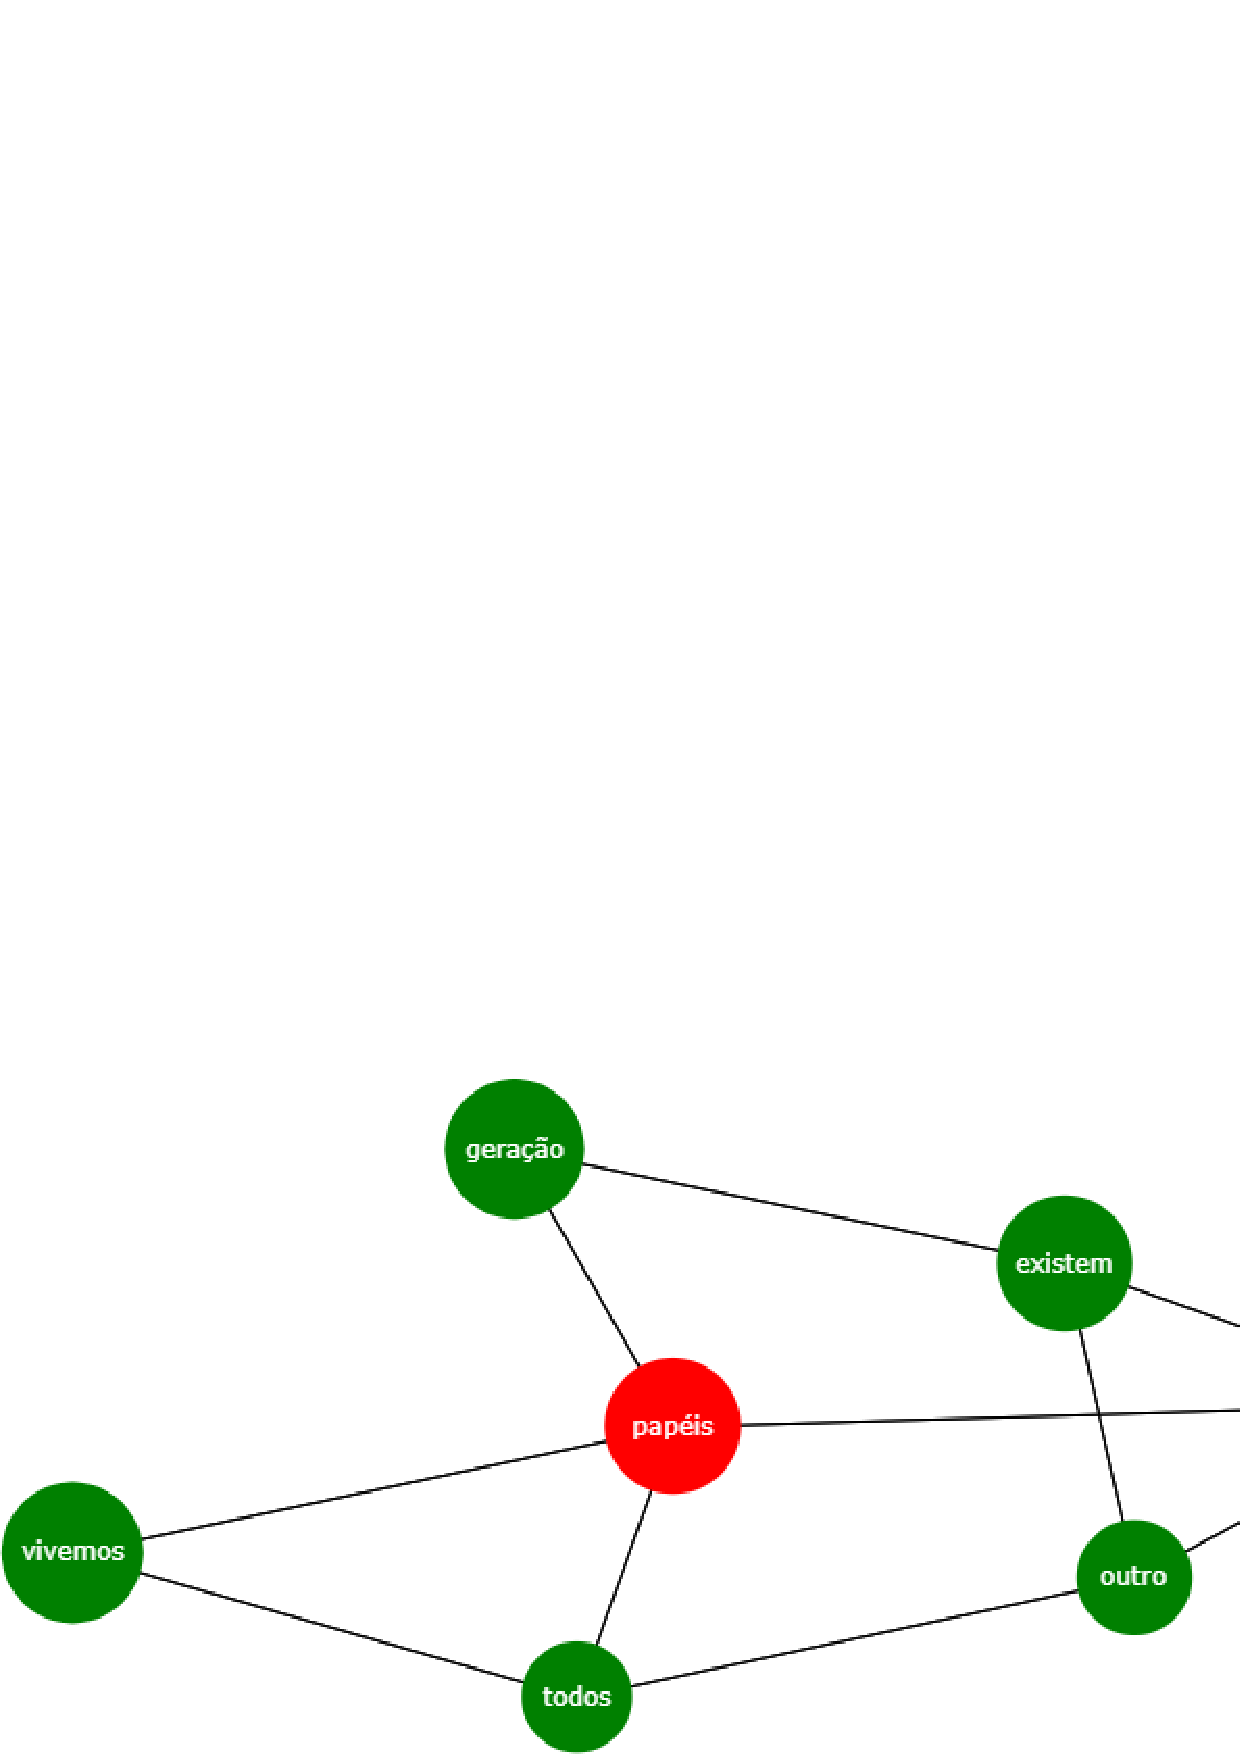
\includegraphics[width=\textwidth]{figures/figure07.jpg}
\caption{Transposição do exercício para a folha de desenho.}
\label{fig-07}
\source{Elaboração própria.}
\end{minipage}
\end{figure}

Várias vezes, quando a professora perguntava se tinham dificuldade em
simular o exercício no Q3DM, os alunos respondiam que não. Eles também
demonstravam um comportamento descontraído e motivado para a
aprendizagem com o auxílio das simulações computacionais.

Os procedimentos facilitaram a construção dos sólidos geométricos no
Q3DM adaptado para o \textit{smartphone}. Foi possível perceber a conexão do Q3DM
com os rapazes, pois rapidamente conseguiram construir os sólidos
geométricos e manipular suas ferramentas. Os rapazes demonstraram
curiosidade em descobrir mais funcionalidades do Q3DM, em comparação com
as moças, que mostraram algum receio em manipular o \textit{smartphone} e
executavam apenas o que a professora solicitava.

Para a mediação do estudo das SCs, os alunos apresentaram-se atentos e
motivados em aprender a simular exercícios no GeoGebra o que facilitou a
comparação do exercício no \textit{smartphone} e na folha de desenho. (Ver \Cref{fig-08}).

\begin{figure}[htpb]
\centering
\begin{minipage}{.5\textwidth}
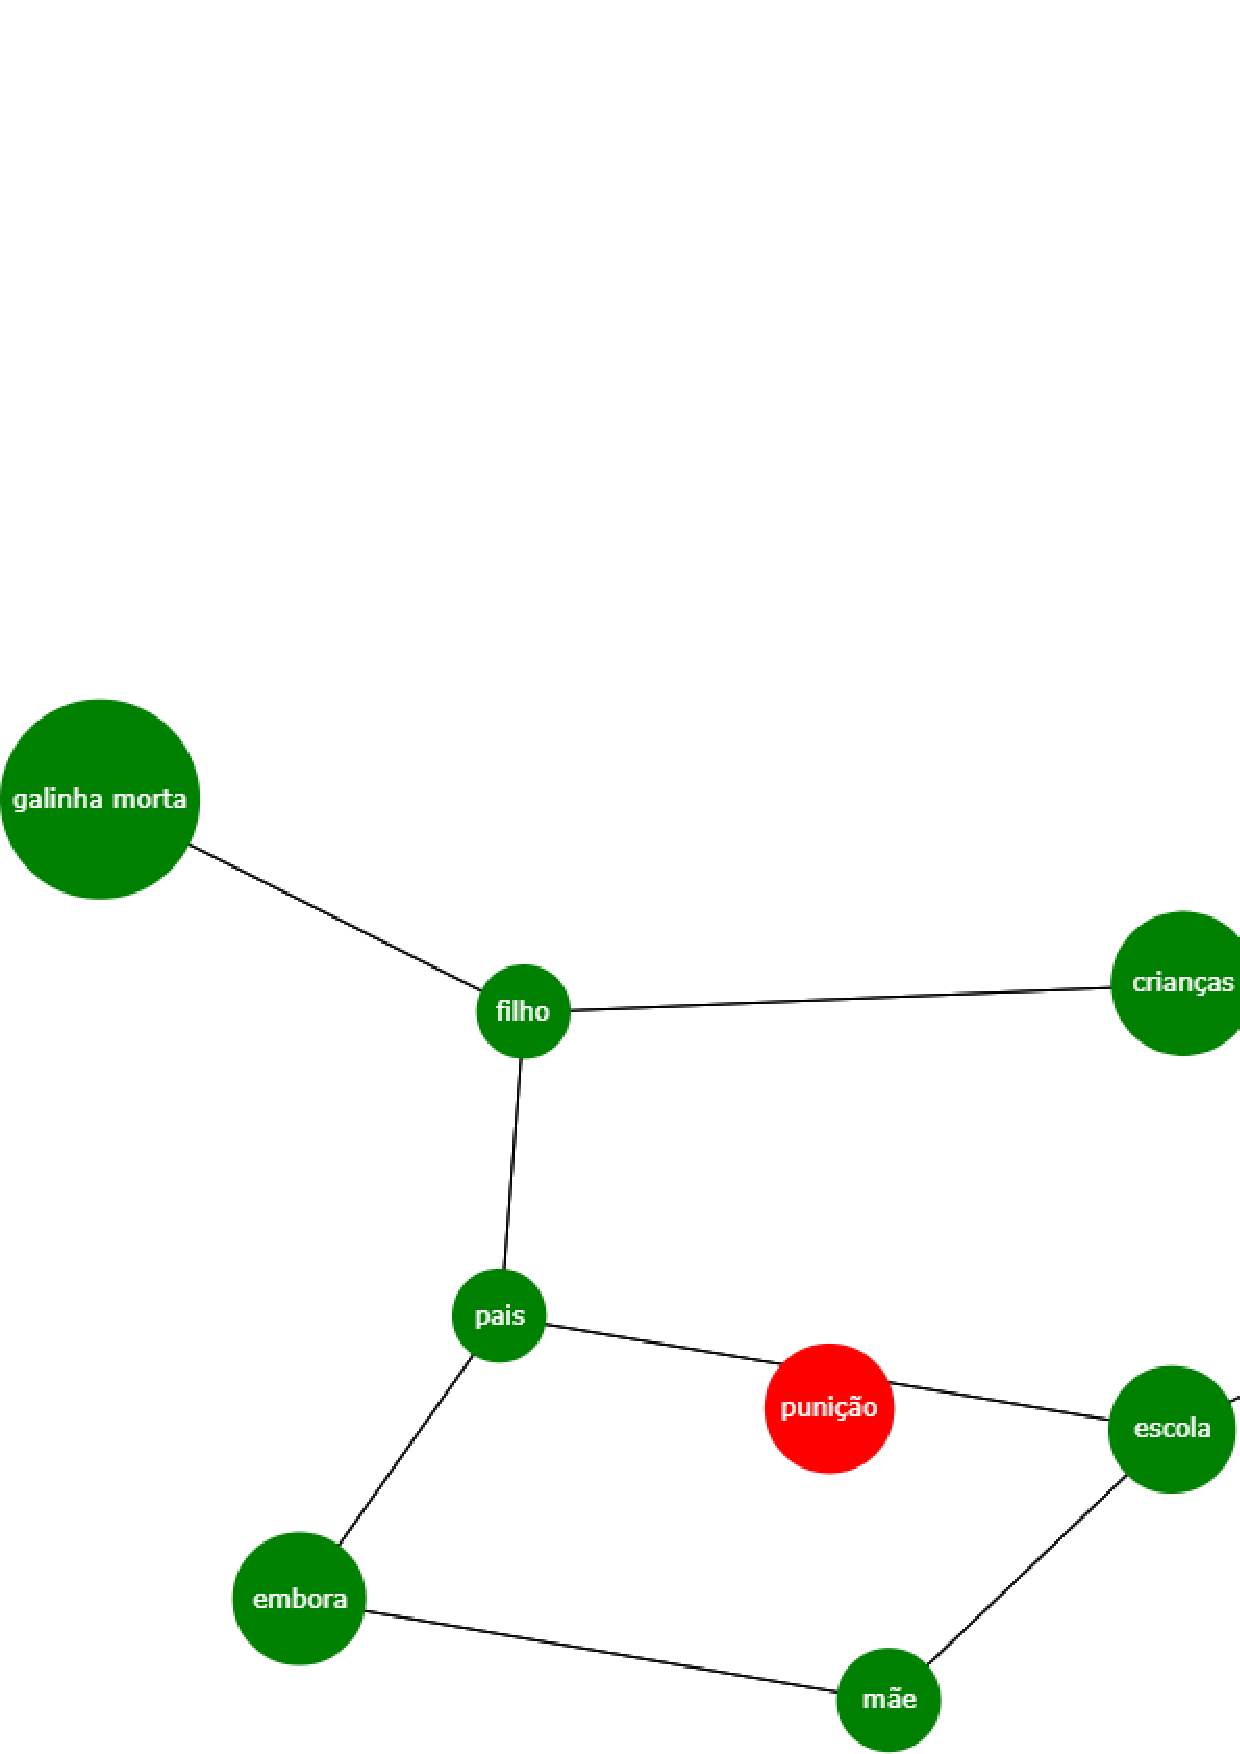
\includegraphics[width=\textwidth]{figures/figure08.jpg}
\caption{Exercício no \textit{smartphone} e na folha de desenho.}
\label{fig-08}
\source{Elaboração própria.}
\end{minipage}
\end{figure}


Foi notável uma semelhança no comportamento dos alunos: uma conexão com
a tecnologia e sua facilidade em compreender os conteúdos abstratos das
POs e SCs. A respeito disso, \textcite[p. 145]{jesus2019}, em seu estudo,
argumentaram que \enquote{quando estudamos geometria descritiva sem o uso do
	GeoGebra, percebe-se a dificuldade em organizar e visualizar o que está
	sendo solicitado pelo professor, assim, acaba provocando desinteresse e
	insucesso do aluno}. Concordando com os autores, foi notório que, na
primeira parte da aula, os alunos demonstraram dificuldade em
compreender os conteúdos teóricos, mas, após a apresentação do AT e dos
procedimentos para a sua manipulação, eles demonstraram uma mudança de
comportamento e mostraram-se motivados em manipular a AT, o que
facilitou a mediação da professora no processo de ensino e aprendizagem.
Esses resultados são coerentes com os encontrados em vários estudos, nos
quais os grupos experimentais desenvolveram competências de visualização
espacial, por terem utilizado a tecnologia \cite{carbonell2017,lukaszewicz2018,omar2019}.

Foi observada uma conformidade nos dois temas(PO e SC): os alunos
demonstraram motivação em explorar mais conteúdos relacionados à aula, o
que permitiu o desenvolvimento de habilidades de VE. Também foi notável,
nos alunos, um comportamento diferente entre os gêneros. Os rapazes
mostraram interesse em explorar os Recursos Tecnológicos e descobrir
mais funcionalidades dos ATs, enquanto as moças tendiam a apenas seguir
as instruções da professora com uma certa timidez, sem explorar
totalmente o potencial das ferramentas. Esse comportamento pode ser
comparado com o estudo de \textcite{fiantika2018}, no qual os autores
concluíram que os gêneros têm comportamentos diferentes na resolução de
problemas geométricos que requerem a VE. Enquanto os rapazes utilizam
geralmente a atividade mental, imaginando objetos espaciais 2D e 3D, as
moças, de forma geral, focam-se em desenhar esboços e criar esquemas 2D.
Isso sugere que a timidez das alunas pode ter a ver com a dificuldade de
VE em 3D, enquanto os rapazes têm mais capacidade de relacionar o 2D com
o 3D.

\subsection{Análise do questionário de satisfação}\label{sub-sec-Análise do questionário de satisfação}

Para a análise dos questionários de satisfação da utilização do Q3DM e
GeoGebra, foram extraídas 3 categorias designadas: modelo de ensino,
ações positivas da aula e ações negativas da aula. No estudo da
aplicação de Q3DM, as descrições ilustraram que a simulação facilitou a
resolução dos exercícios das POs, por meio da sua interface, o que
permitiu a visualização detalhada dos sólidos e a sua respectiva
construção. As respostas indicaram que, além da sua facilidade, o AT foi
seguro. Reiteraram que o modelo de aula com o auxílio do Q3DM pode
auxiliar a resolução dos exercícios de forma rápida e prática, e não
requer muito trabalho. Destacaram a importância da simulação do Q3DM
pela sua eficiência de utilização e pela visualização das vistas
ortogonais.

Quanto ao estudo da aplicação do GeoGebra, as descrições dos alunos
nortearam que o aplicativo, além de motivar a aprendizagem, facilita a
resolução dos exercícios. Afirmaram que o modelo tradicional é mais
difícil em comparação com o modelo com auxílio da tecnologia. Não
obstante, certificaram que o uso do GeoGebra foi benéfico pela sua
facilidade de simulação e promoção da VE na aprendizagem da seção do
cilindro. Referiram, ainda, que a simulação permite construir, de forma
rápida, os elementos da GD, o que impulsionou a percepção da dinâmica
dos sólidos no espaço e a sua comparação com as representações na folha
de desenho. Alegaram que é vantajoso usar o GeoGebra, porque promove a
imaginação em 3D e a percepção das seções de acordo com a posição do
plano no sólido. Confirmaram que o AT facilitou a projeção das figuras e
a leitura das VOs de forma detalhada. Argumentaram que o GeoGebra
possibilitou a construção de pontos, retas e outros elementos
necessários para GD, o que tornou a aprendizagem mais facilitada. Esses
resultados estão alinhados com o estudo de \textcite{silva2017}, no
qual os autores afirmaram que os alunos ficaram animados com a dinâmica
de ATs, se propuseram a fazer o download em casa e a investigar as suas
funcionalidades. Isso sugere que os ATs podem ser um potencial para
facilitar a aprendizagem dos alunos.

Quanto às descrições dos aspectos positivos da aula, os alunos do estudo
da aplicação do Q3DM evidenciaram que a aprendizagem foi facilitada pela
boa mediação da professora. Houve motivação e gosto pela aprendizagem,
possibilitando a construção dos sólidos no Q3DM. Isso incluiu a
modelagem de sólidos, inclusive os complexos, com facilidade de
representações. A percepção rápida dos alunos foi evidente, assim como a
facilidade de visualização das vistas ortogonais. Eles demonstraram
aprendizado das POs e facilidade em manusear o Q3DM, revelando um gosto
pelo software. A facilidade de percepção da visualização dos sólidos em
3D também foi notável.

Relativamente ao estudo da aplicação do GeoGebra, as respostas
clarificaram que houve boa mediação e paciência por parte da professora,
o que facilitou a construção de sólidos que antes os alunos não
conseguiam realizar. A mediação da professora tornou os exercícios mais
fáceis, promovendo a facilidade de aprendizagem e motivando os alunos a
aprender. Eles demonstraram percepção rápida durante o estudo do
cilindro e na manipulação do GeoGebra. A construção do cilindro no
GeoGebra permitiu aprofundar os conteúdos das seções, promovendo a
visualização espacial e a projeção de sólidos. A simulação no GeoGebra
também contribuiu para a promoção do conhecimento dos conteúdos da
Geometria Descritiva, tornando-o um excelente aplicativo para abordar a
GD.

No que se refere aos aspectos negativos na aula do estudo da aplicação
do Qubism 3D Modeling, as descrições apresentam que, no decorrer da
aula, não foi identificado nenhum aspecto negativo. Os alunos não
apresentaram dificuldades e nenhum problema foi relatado. No entanto, no
início da aula, houve uma situação em que foi complicada a compreensão
da VE sem o auxílio da tecnologia, mas foi rapidamente resolvida.

Em relação ao estudo da aplicação do GeoGebra, os alunos afirmaram que,
no início da aula, parecia que tudo seria difícil, e o tempo disponível
para a resolução do exercício acabou sendo curto. Além disso, os alunos
acharam o exercício um pouco difícil e requereram muita concentração
para completá-lo.

Desse modo, dos resultados obtidos nas 3 categorias, fez-se a análise
das frequências das palavras e a categorização indutiva para obter uma
compreensão da pesquisa que foi desenvolvida em torno da pergunta de
pesquisa deste estudo. Constatou-se que os alunos tiveram facilidade
para resolver os exercícios das POs/SCs. Através da sua interface,
permitiu-se a construção dos sólidos e a sua visualização detalhada. As
definições também indicaram que, além dos aplicativos possibilitarem a
facilidade de construção dos elementos geométricos, o modelo de aula com
o auxílio da tecnologia auxilia a resolução dos exercícios de forma
rápida e prática.

Os ATs auxiliam no processo de aprendizagem, porque não só é fácil de
manusear, como também é interativo, permitindo ao aluno uma mudança
imediata de ponto de vista, aumentando a compreensão dos sólidos
geométricos \cite[p. 220]{mexas2015}. Corroborando os autores e
aliando as definições acima apresentadas, as simulações dos ATs
(Q3DM/GeoGebra) são eficientes para a aprendizagem de representações em
3D.

De modo geral, as definições apresentaram a resposta da pergunta de
pesquisa que é: através da eficácia da realização das simulações
computacionais de aplicativos adequados aos conteúdos das POs e Scs.,
porque os aplicativos, além de terem motivado a aprendizagem,
facilitaram a resolução dos exercícios, promoveram a VE dos sólidos de
forma rápida e impulsionaram a comparação das representações nos
aplicativos com as representações na folha de desenho. Esses resultados
podem ser comparados com os resultados do estudo de \cite[p. 154]{qin2018},
que argumentam que, para melhorar a qualidade da aprendizagem, é
necessário mudar o modo tradicional de ensino, aplicar novas
tecnologias, reforçar a prática de produção de animação 3D para auxiliar
a melhora da interação entre o professor e o aluno.

Durante a realização do questionário, os alunos apresentaram-se
motivados e responderam rapidamente. Os alunos resolveram o problema
prático de forma interativa e colaborativa. Apesar da simulação com o
uso da tecnologia, o professor continua sendo o agente mediador dos
conteúdos, responsável por selecionar a tecnologia adequada ao ensino,
avaliador do processo de ensino e aprendizagem. Isso significa que o
professor é quem faz as intervenções pedagógicas com uso das
tecnologias, planeja, organiza e conduz a mediação para sucesso-processo
do processo de aprendizagem do aluno \cite{zanatta2015}. Na
mesma linha de pensamento com os autores, concordamos que o professor
continua sendo o orientador do processo de ensino e aprendizagem.
